\documentclass[a4paper,preprintnumbers,aps,citeautoscript,notitlepage,12pt,tightenlines]{revtex4-2}
\usepackage[a4paper,margin=0.75in]{geometry}
\usepackage[utf8]{inputenc}
\usepackage[T1]{fontenc}
\usepackage{microtype}
\usepackage[italian]{babel}
\makeatletter
\let\it@comma@def\active@comma
\makeatother
\usepackage{physics}
\usepackage{graphicx}
\begin{document}
\count\footins = 1000
% \preprint{LMCS\_d0\_\today}
% \preprint{Electromagnetic-Waves-003/1}
\title{Misura delle righe di Balmer per H con metodi Monte Carlo}
%\author{A. Parodi}
\author{F. Polleri}
\author{M. Sotgia}
\email{s4942225@studenti.unige.it}
\affiliation{Dipartimento di Fisica, Università degli Studi di Genova, 16146 Genova, Italy}
\date{\today}
% \revised{\today}
\maketitle

\section{Introduzione}
Un prisma ottico può essere utilizzato, sfruttando il fenomeno della rifrazione, come spettrometro per eseguire misure precise della lunghezza d'onda dato un fascio monocromatico incidente, in grado anche di separare le componenti di un fascio non monocromatico. 

Si sa che infatti la differenza $\delta_i$ tra l'angolo in ingresso $\theta_0$ e l'angolo in uscita $\theta_i$ risulta essere legato al valore dell'indice di rifrazione del materiale, \begin{equation}\delta_i = \theta_0 - \alpha+\arcsin\left(n\sin\left(\alpha - \arcsin\left(\frac{\sin\theta_0}{n}\right)\right)\right),\end{equation} con $n$ indice di rifrazione e $\alpha$ apertura angolare del prisma. 

Si osserva che $\delta_i$ ha un minimo in corrispondenza del quale la misura è più stabile e la relazione precedente si semplifica come \begin{equation} n\sin\frac{\alpha}{2} = \sin\frac{\delta_m + \alpha}{2} = \sin\theta_{0_m}.\end{equation}

Da quest'ultima relazione possiamo ottenere una forma per l'indice \begin{equation} n(\theta, \theta_0) = \frac{\sin\frac{\theta-\theta_0 + \alpha}{2}}{\sin\frac{\alpha}{2}}.\end{equation}

Possiamo anche però ricavare la relazione che lega l'indice di rifrazione $n$ al valore di $\delta_m$, e poichè $n=n(\lambda)$, secondo la relazione di Cauchy \begin{equation} n(\lambda) = A + \frac{B}{\lambda^2},\end{equation} appropriata ad un ordine $\mathcal O (1/\lambda^2)$, con $A$ e $B$ coefficienti propri del materiale in questione, allora possiamo concludere che esistono relazioni che legano $\lambda$ con il valore di $\delta_i$. 

\subsection{Angoli di Balmer}

Data la lunghezza d'onda, in cui si osservano rispetto ad un elemento le bande di assorbimento o di emissione, viene definita da Balmer una relazione che permette di quantificare la posizione di queste bande \begin{equation} \frac{1}{\lambda} = R_H \qty(T(n) - T(m)) \end{equation} che nel caso dell'idrogeno assume una forma particolarmente comoda, dove $T(n) = 1/n^2$. Otteniamo quindi una equazione del tipo \begin{equation} \frac{1}{\lambda} = R_H \qty(\frac{1}{n^2} - \frac{1}{m^2}). \end{equation}

\section{Misura della costante di Rydberg}

Un utilizzo che possiamo fare delle relazioni fino ad ora trovate, e dello strumento che abbiamo descritto, è quello di sfruttarlo per ottenere una stima del parametro $R_H$, detto costante di Rydberg, dalla relazione degli angoli di Balmer. Sono noti gli angoli $\theta_i$ ai quali si trovano le bande di emissione dell'idrogeno, per $m = 3, 4, 5, 6$ e $n=2$, e si conoscono i parametri $A$, $B$ con le loro distribuzioni e il coefficiente di correlazione che esiste tra i due, $\rho_{AB}$. 

\begin{figure*}
\centering
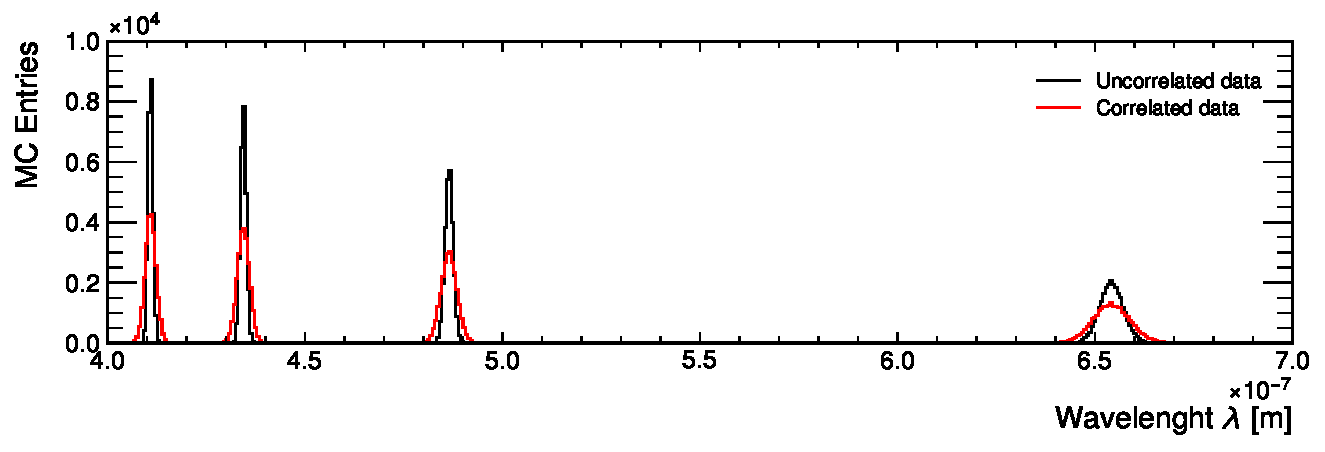
\includegraphics[width=\linewidth]{../tasks/wavelenght}
\caption{}
\end{figure*}

\end{document}